% File hicss51.tex
%%
%% Based on the style files for ACL 2015 by 
%% car@ir.hit.edu.cn, gdzhou@suda.edu.cn


\documentclass[10pt]{article}
\usepackage[letterpaper]{geometry}
\usepackage{hicss}
\usepackage{times}
\usepackage[none]{hyphenat}
\usepackage{url}
\usepackage{latexsym}
\usepackage{minted}
\usepackage{indentfirst}
\usepackage{graphicx}
\graphicspath{{images/}}
\usepackage[
    style=apa,
  ]{biblatex}
\addbibresource{sample.bib}

\newcommand{\sansserifformat}[1]{\fontfamily{cmss}{ #1}}%

\setlength\titlebox{7cm}

\makeatletter
\AtEveryCitekey{\ifnameundef{shortauthor}{}{\def\cbx@apa@ifnamesaved{\@firstoftwo}}}
\makeatother

% You can expand the titlebox if you need extra space
% to show all the authors. Please do not make the title box
% smaller than 5cm (the original size).

\usepackage{booktabs}
\usepackage{enumitem}
\usepackage{hicss}


\addbibresource{references.bib}
% \bibliographystyle{apalike}
% \bibliography{sample}
\bibliography{references}

\title{Addressing Challenges in a Dangerous World: Developing a Design Science Artifact for Advancing Open Source Intelligence (OSINT) Research}
%Mission Critical in a Dangerous World: Developing a Literature-Based Foundation for Better Open Source Intelligence (OSINT) Research}

\author{Franz Kayser\\
ESG \\
 {\underline{ franz.kayser@esg.de}} \\\And
 Dr. Thomas Mayer \\
 ESG \\
 {\underline{ thomas3.mayer@esg.de} }\\\And 
 Prof. Dr. Michael Bücker \\
University of Applied Sciences Münster\\
 {\underline{michael.buecker@fh-muenster.de}} \\}
  
\date{}


\begin{document}
\maketitle
\begin{abstract}
    Open Source Intelligence (OSINT), which derives intelligence from public data, has gained attention since the Russian invasion of Ukraine. Despite attempts at standard definitions, research on technology-driven intelligence gathering remains ambiguous. This paper employs a Design Science Research (DSR) approach to categorize this construct. Analyzing sixty studies through a structured literature review, three domains were identified: maturity, Intelligence Cycle (IC) phase, and use case. The resulting framework, developed into a trend radar (TR), was evaluated with expert interviews, revealing technological gaps in the planning/direction and dissemination/integration phases. Although intelligent support technologies exist, practical implementation lags behind theory, with the human factor remaining central to OSINT. Findings suggest future research should focus on developing applications for underserved phases and investigating why proven solutions are not widely adopted, considering legal, ethical, political, and social factors. This study contributes to the literature by providing a knowledge base, identifying research gaps, and guiding further research.
    %Open Source Intelligence (OSINT), the process of gathering intelligence from public data, is under intense scrutiny, heightened since the Russian invasion of Ukraine. However, despite numerous attempts at standardized definitions, the research contexts around the topic of technology-driven intelligence gathering and analysis   remains ambiguous. This paper addresses this gap by using a Design Science Research (DSR) approach to develop a systematic  categorization  of the technology-driven intelligence construct. Sixty studies were analyzed using structured literature review. This approach yielded three domains: maturity, IC phase, and use case. This framework, developed into an artifact as a trend radar, was evaluated using expert interviews. The process revealed technological gaps in the planning/direction and dissemination/integration phases. Although intelligent support technologies were identified, practical implementation lags behind theory. And importantly, the human factor remains central to the OSINT process. The findings of this study suggest future research should develop applications for underserved phases and examine why proven applications are not widely adopted, focusing on legal, ethical, political, and social factors. Thus, the study contributes to the literature on technology-driven intelligence by serving as a knowledge base, and tool for identifying research gaps, and a guide for further research.
\end{abstract}

\section{Introduction} \label{sec:introduction}

OSINT, the process of extracting intelligence from public data (\cite{DosPassos.2017}), has gained attention, especially since the 2022 Russian invasion of Ukraine. Real-time analysis of social media has proven pivotal in uncovering valuable insights (\cite{SmithBoyle.24.07.2023}). Despite numerous attempts to define OSINT (\cite{PastorGalindo.2020, Yogish.2021}), controversy persists due to ongoing advancements in computer and data sciences that continuously enhance collection and analysis capabilities (\cite{Ghioni.2023}).

The surge in open communication channels has led to an 'information explosion' (\cite{Hwang.2022}), making previously restricted data publicly accessible (\cite{Williams.2018}) and reshaping intelligence paradigms (\cite{Dokman.2020}). However, fundamental scientific literature in the field remains limited (\cite{HerreraCubides.2020}), failing to keep pace with rapid developments (\cite{Ghioni.2023, Williams.2018}). Key questions regarding the existence of autonomous third-generation OSINT systems remain unanswered (\cite{Ghioni.2023, PastorGalindo.2020}), and OSINT use cases unexplored (\cite{AlKilani.2021, Ghioni.2023}), largely due to the challenges in accessing government and security sectors (\cite{HerreraCubides.2020, PastorGalindo.2019}).

A robust, structured framework is needed to enhance the scientific understanding and application of OSINT. This study addresses the research question: \textit{How can current OSINT trends, in the form of technologies and their characteristics, particularly maturity levels and use cases, be presented in a unified way that bridges academic research and practical applications?} This paper investigates current OSINT trends using the DSR approach (\cite{Peffers.2007}). The method involves a systematic review (\cite{Cleven.2009}) to analyze OSINT literature, establishing a unified knowledge base.
OSINT technologies and their characteristics will be visualized in a TR, evaluated through semi-structured interviews (\cite{Glaser.2009}) with German security experts, and analyzed via qualitative content analysis (\cite{Billings.1997}). The research background material is available on GitHub (\cite{kayser2024}).
%OSINT technologies and their characteristics will be visualized in a TR, evaluated through semi-structured interviews  with security sector experts in Germany, and analyzed using qualitative content analysis . 


\section{Theoretical Background} \label{sec:theoreticalbackground}

%The domain of OSINT is continuously expanding due to the ongoing improvements of collecting and analysis possibilities \cite{Ghioni.2023, Williams.2018}. In addition, the new means and methods of communication associated with advances in information and communication technology have turned OSINT into a complex discipline \cite{Benes.2013, Williams.2018}.

\subsection{Open Source Intelligence}

One of the earliest referenced definitions
was published by the North Atlantic Treaty Organization (\textcite{NorthAtlanticTreatyOrganization.2001}): \textit{"OSINT is information that has been
    deliberately discovered, discriminated, distilled, and disseminated to a selected audience,
    [...], in order to address a specific question. OSINT, [...] thus applies the proven
    process of intelligence to the broad diversity of open sources [...] and creates
    intelligence."} However, today the discipline is no longer seen as a purely governmental
matter. Private research institutions and organizations (\cite{Bohm.2021}) are
also massively driving the development of such systems
(\cite{Dokman.2020}). The focus is shifting to
developing OSINT into third-generation robust, autonomous solutions (\cite{PastorGalindo.2019}).

\subsection{Intelligence and Intelligence Cycle}

OSINT's core task is to generate decision-making intelligence
(\cite{NorthAtlanticTreatyOrganization.2001}). The generation process of such an intelligence product
is referred to as the IC specified by the Central lntelligence Agency (\cite{CentralIntelligenceAgency.1987}).
It represents the central element of every intelligence discipline (\cite{Reuser.2017}).
The link between the phases is that the result of each preceding phase serves as input for the subsequent phase, following the U.S. Joint Force Command (\cite{JointChiefsofStaffU.S.Army.2013}), continuously iterated to meet new requirements (\cite{Gibson.2016}).
Today, to represent external influences or assign responsibilities (\cite{Lowenthal.2020,Phythian.2013}), numerous
variations can be found (\cite{Reuser.2017}). The IC should hence be seen less as a guideline and more as an informal
coordination element (\cite{Hwang.2022}). \textcite{JointChiefsofStaffU.S.Army.2013} segmented the cycle into six phases (Figure \ref{fig: Intelligence Cycle}).

\begin{figure}[h]
    \centering
    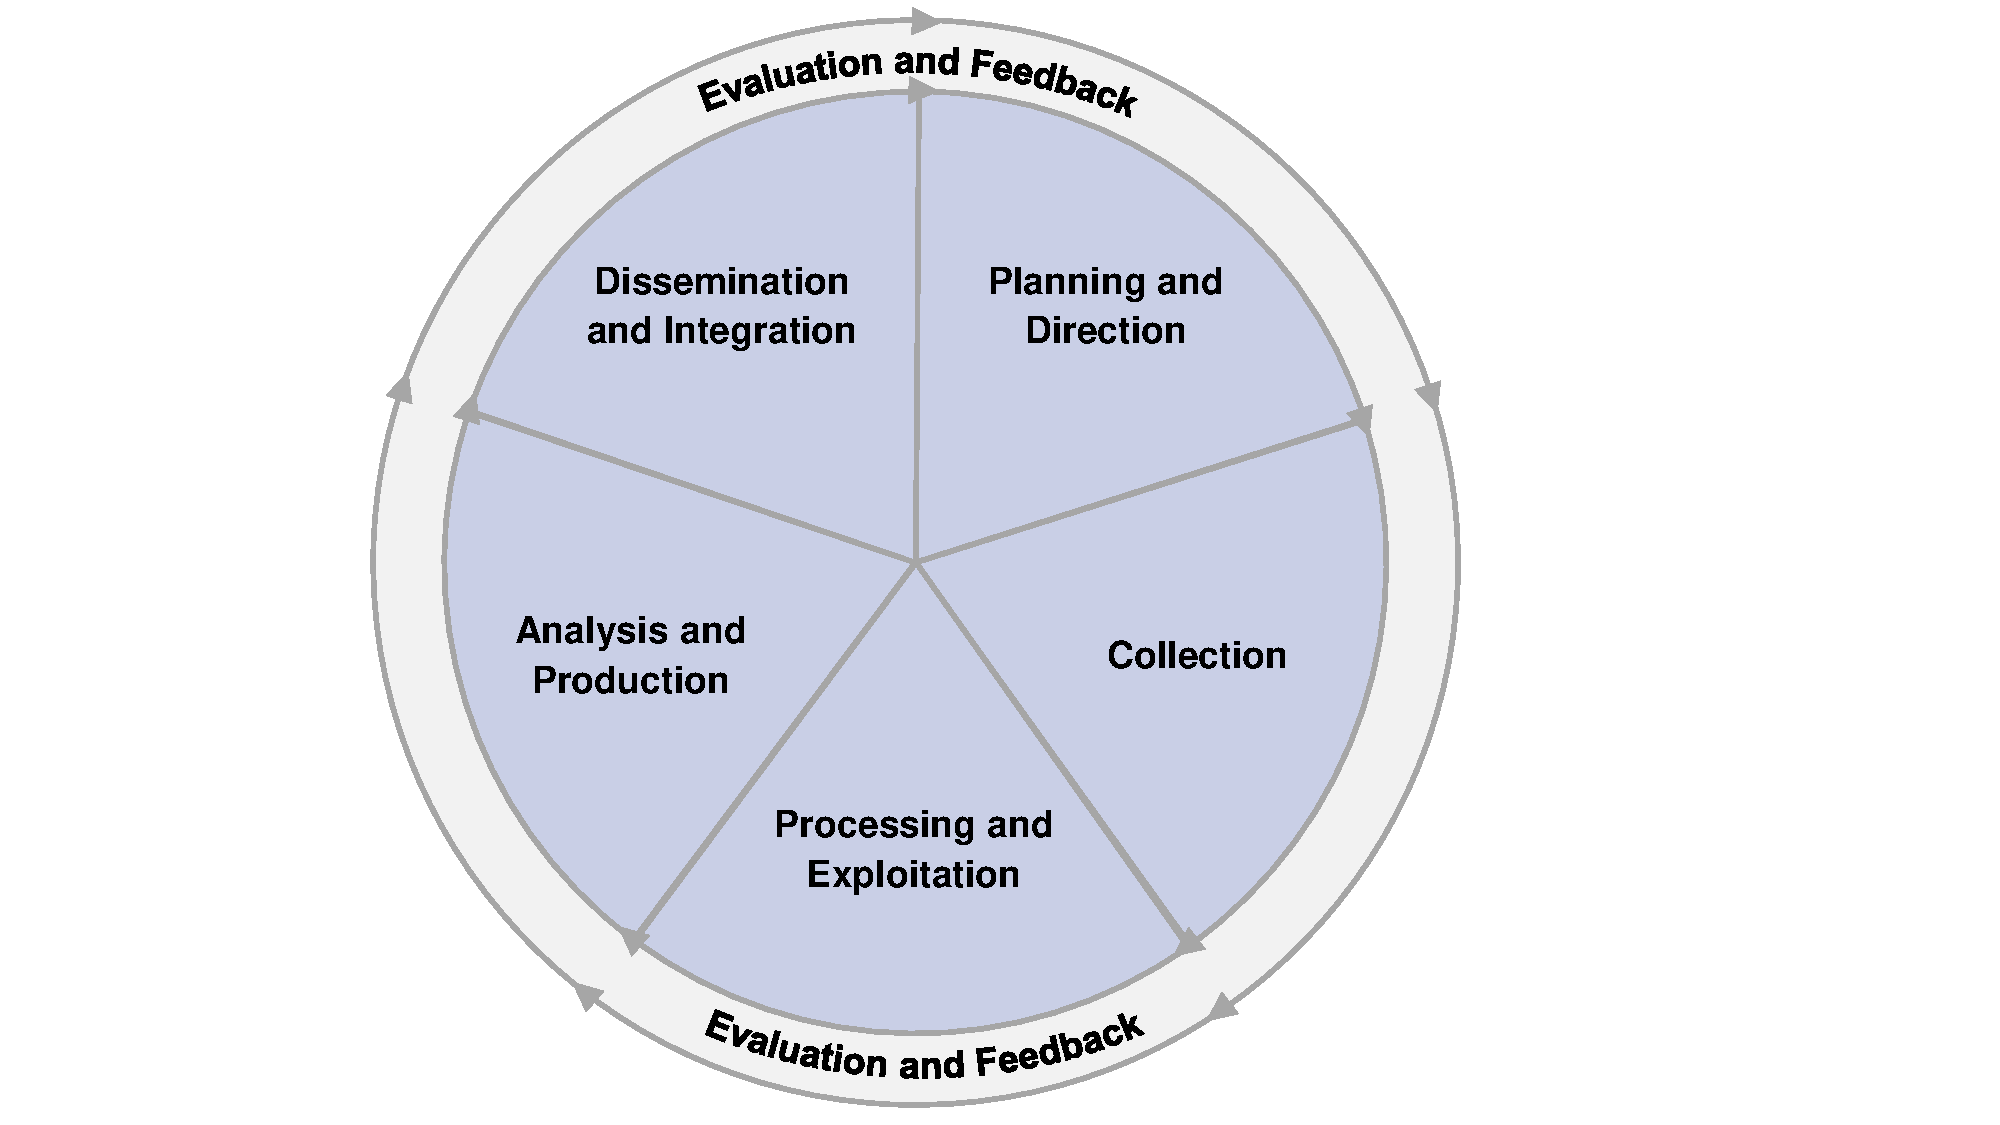
\includegraphics[clip,width=0.6\linewidth]{PDF/images/crop_Intelligence Cycle}
    \caption{Intelligence Cycle (\textcite{JointChiefsofStaffU.S.Army.2013})}
    \label{fig: Intelligence Cycle}
\end{figure}

The planning/direction phase combines the identification, definition, prioritization, and monitoring
of the requirements (\cite{JointChiefsofStaffU.S.Army.2013}).
The collection phase refers to the gathering of raw data (\cite{CentralIntelligenceAgency.1987}).
It consists of iterative repetition of research
(\cite{NorthAtlanticTreatyOrganization.2001}) to make the query more precise with each run
(\cite{PastorGalindo.2020}). The processing/exploitation phase involves condensing
these data volumes into action-relevant information
(\cite{JointChiefsofStaffU.S.Army.2013}).
Analysis/production refers to the synthesis of the information obtained into a timely and accurate intelligence product
(\cite{NorthAtlanticTreatyOrganization.2001}).
The final phase consists of handing over the product to the 'customer' in a
usable form (\cite{CentralIntelligenceAgency.2023, Williams.2018}).
Evaluation/feedback are not to be regarded as individual phases
but take place continuously to achieve progressive optimization
(\cite{JointChiefsofStaffU.S.Army.2013, NorthAtlanticTreatyOrganization.2001}).

\subsection{Previous Studies}

Eight publicly accessible literature reviews exist on OSINT. \textcite{DosPassos.2017} showed how big data and data science enhance decision-making. \textcite{PastorGalindo.2019, PastorGalindo.2020}
provided insights into OSINT's state, focusing on cyber security
enhancements. They conducted the first rudimentary mapping of OSINT trends, observing its use in social opinion and sentiment
analysis, cyber crime and organized crime, as well as cyber security and cyber defense. \textcite{GarciaLozano.2020} identified methods for computer-assisted veracity assessment of public information, while
\textcite{HerreraCubides.2020} researched the production of research/educational materials. They concluded that OSINT
publications are less common compared to other trending topics. \textcite{Yogish.2021} explored AI  implementation in cyber security, showing its potential to simplify OSINT given increasing data volumes.
\textcite{Hwang.2022} investigated security threats and cyber criminality through OSINT misuse.
\textcite{Ghioni.2023} examined the political, ethical, legal, and social implications of
OSINT in conjunction with AI, highlighting the absence of a comprehensive framework and the early stage of third-generation OSINT.

\section{Research Methodology}

The study follows the iterative DSR approach, a theory-based research paradigm for developing a directly applicable solution in the form of an innovative artifact (\cite{vomBrocke.2020b})
to solve a (practical) problem (\cite{Peffers.2007}). Hence, the model is ideal for creating an artifact to address the definitional gap and lack of academic frameworks. %Hence, the model is ideally suited for creating an artifact that can be useful for addressing the aforementioned definitional gap and lack of academic frameworks. 
The DSR methodology includes six successive activities (\cite{Peffers.2007}, Figure \ref{fig: DSRM}). Section \ref{sec:introduction} summarizes step 1, while steps 2-5 will be discussed in detail in sections \ref{sec:designobjectives}-\ref{sec:eval}. Sections \ref{sec:results} and \ref{sec:discussion} present the outcomes of step 6. Continuous evaluation of steps 1-4 occurred throughout the study following \textcite{Sonnenberg.2012}.

\begin{figure*}[thb]
    \centering
    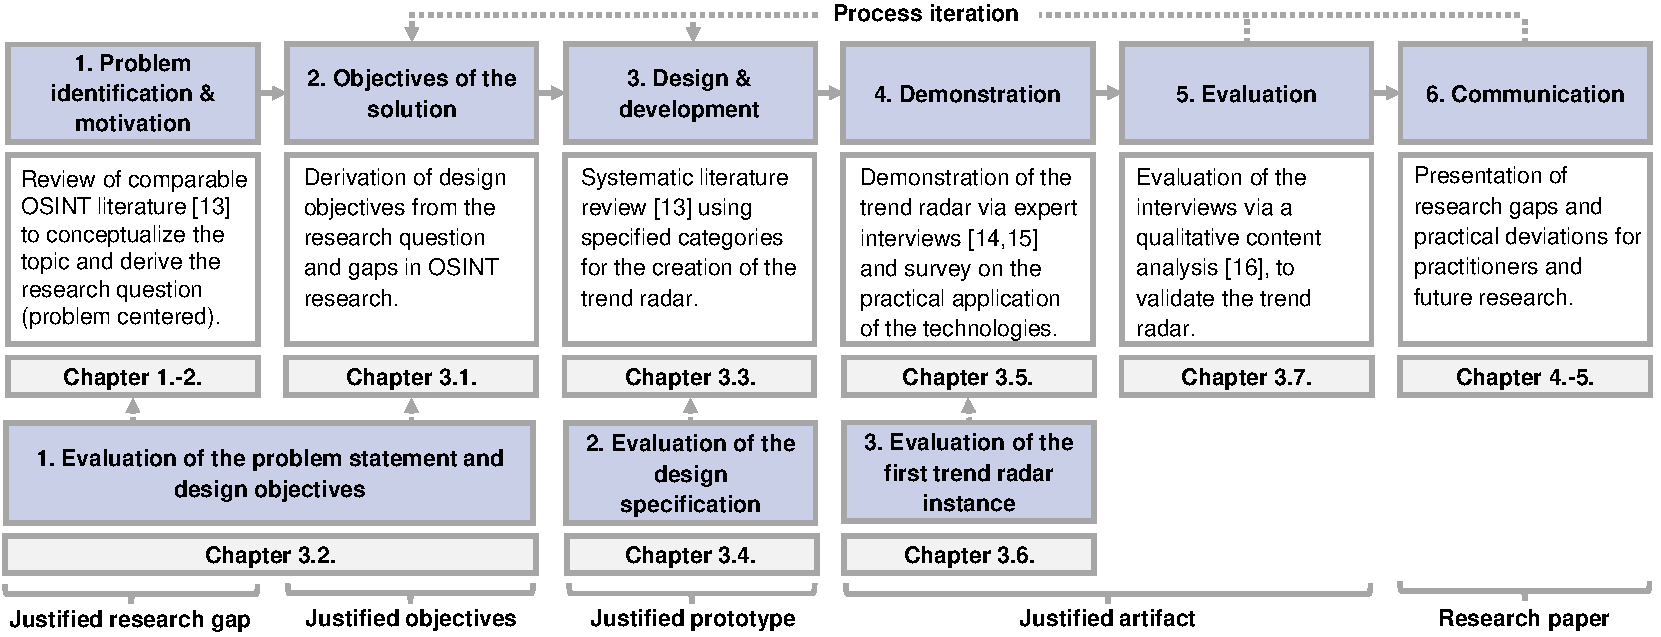
\includegraphics[width=0.7\textwidth]{PDF/images/cropped DSR_V01.pdf}
    \caption{Iterative DSR model (\cite{Peffers.2007}) with control steps (\cite{Sonnenberg.2012})}
    %DSR is a theory-based iterative approach for developing innovative solutions (\cite{Peffers.2007}). It involves six steps and includes three control steps (\cite{Sonnenberg.2012}) for continuous refinement.
    \label{fig: DSRM}
\end{figure*}

\subsection{Design Objectives of the Solution} \label{sec:designobjectives}


The design objectives, derived from the research question (\cite{Peffers.2007}), are categorized into content-related (CO) and formal objectives (FO).

\setlist{noitemsep}
\begin{itemize}
    \item[\textbf{CO1:}] Third-generation OSINT systems remain unconfirmed (\cite{Ghioni.2023}). The artifact must reflect the intelligence generation process to map technologies by usage to respective phases and identify research gaps.
        %The artifact must mirror the intelligence generation process, facilitating structured mapping of identified technologies based on their usage. This enables direct assignment of research gaps to respective phases, verifying the existence of third-generation OSINT systems.
    \item[\textbf{CO2:}] Key use cases (\cite{AlKilani.2021, Dokman.2020, Ghioni.2023}), technologies, and their characteristics are lacking in OSINT research (\cite{Ish.2022}). The artifact must include technology maturity to inform research status and use cases to indicate research directions.
        %Key characteristics, such as technology maturity levels and use cases, must be considered. Technology maturity informs research status, while use cases reveal research directions.
    \item[\textbf{FO1:}] Given OSINT's rapid evolution (\cite{Ghioni.2023}), the artifact requires a simple, standardized structure to quickly identify research gaps and ensure cross-disciplinary applicability.
        %The artifact must follow a simple structure for quick identification of research gaps and high standardization for applicability across intelligence disciplines.
    \item[\textbf{FO2:}] Due to the high field dynamic, predicting future developments is challenging (\cite{Benes.2013}). The artifact should be designed for continuous expansion to remain relevant over time.
        %The artifact should be continually expandable to capture field dynamics effectively.
\end{itemize}

\subsection{Evaluation of the Problem Statement and Design Objectives} \label{sec:eval}
In section \ref{sec:theoreticalbackground}, the theoretical background of the research is outlined, focusing on the IC, which is crucial for the artifact's development. The artifact is evaluated for its compatibility within the OSINT framework. Additionally, the review of prior studies highlights a significant gap in comprehensive OSINT research, emphasizing the inquiry's importance and relevance.

\subsection{Design and Development}
The third activity is a systematic literature review, guided by \textcite{Cleven.2009}.  The taxonomy by \textcite{Cooper.1988} scoped the review, setting up classification categories for concept matrices to structure the literature analysis (\cite{Webster.2002}).
To standardize verification across the IC, general categories reflecting established technology evaluation criteria were defined for each phase, except the iterative evaluation/feedback phase. For the collection phase, six categories were developed:
\setlist{noitemsep}
\begin{itemize}
    \item \textbf{Use case:} Application areas of the technologies.
    \item \textbf{Data:} Composition and types of data foundations, including data format and source.
    \item \textbf{Process:} Degree of automation in the technologies (manual, semi-automated, automated, fully automated; \cite{Duncheon.2002, Billings.1997, Endsley.1999}).
    \item \textbf{Technology:} Material and immaterial means used for managing information (\cite{Bleck.2004}).
    \item \textbf{Technology Complexity:} Assessed through subcategories of volume, variety, and velocity (\cite{Singh.2012}).
    \item \textbf{Maturity Level:} According to the phases innovation, prototype, and  market establishment (\cite{Stich.2022}).
\end{itemize}

Similar categories were adapted for the other phases of the IC, with complexity measured via the analytics spectrum: descriptive, diagnostic, predictive, and prescriptive (\cite{Delen.2013}). The literature search used a broad string ("OSINT" OR "Open Source Intelligence" OR "Open-Source Intelligence" OR "open source intelligence" OR "open-source intelligence"), limited to publications from 2020 to 2023 to capture recent advancements, spanning four databases: Web of Science, IEEE Xplore, ACM Digital Library, and arXiv. A total of 60 studies were analyzed using the SQR3 method (\cite{Robinson.1970}) and organized into a structured Excel spreadsheet for each IC phase.

Technologies were categorized and analyzed for interrelationships within the OSINT framework. Verification was done using a Python script that scanned the papers for predefined keywords. The verified categories and relationships informed the artifact's development based on validated concept matrices.

For this study, a TR was selected as the artifact. This strategic tool identifies, monitors, and evaluates trends affecting industries or organizations, typically using circular diagrams with layers representing relevance or impact (\cite{wulfmettbrenn2017}).

\subsection{Evaluation of the Design Specifications}
The IC forms the foundation of the TR, offering clarity and an intuitive framework that simplifies technology extraction and research gap identification. Its design also ensures applicability across diverse intelligence disciplines in Germany, where this research was conducted. By emulating the structure of the German Federal government's TR (\cite{Stich.2022}), the categories included in this radar have been limited to use case, technology, and maturity level. This focus enhances robustness, user-friendliness, and appropriate detail in the artifact. The concept matrices enable regular updates to the radar, ensuring current and standardized design. Rigorous verification of internal consistency maintains categorization integrity, meeting critical evaluation criteria in contemporary design research (\cite{Sonnenberg.2012}).


\subsection{Demonstration}
The TR was demonstrated via guideline-based, systematizing expert interviews. Particularly in less structured and sparsely linked subject areas, this method enables dense data collection (\cite{Meuser.1991}), especially when access to the social field is limited (\cite{Glaser.2009}).

Experts (Table \ref{tab:experts}) were selected using theoretical sampling (\cite{Glaser.1967}), focusing on Germany, the study's primary country of interest, to evaluate relevant trends. At least one expert from a security authority, the security industry, and a startup was chosen to capture diverse perspectives. A 'prestigious' company position ensures respondents possess relevant research knowledge.

\begin{table*}[hbtp]
    \caption{Interviewed experts}
    \begin{tabular}{p{0.05\linewidth}p{0.2\linewidth}p{0.45\linewidth}p{0.15\linewidth}}
        \toprule
        \textbf{ID} & \textbf{Organization} & \textbf{Position}                      & \textbf{Interview date} \\
        \hline
        E1          & Industry/ Authority   & Senior Intelligence Consultant         & 07-14-2023              \\
        \hline
        E2          & Industry/ Authority   & Referent Corporate Security            & 07-19-2023              \\
        \hline
        E3          & Authority             & In-House Senior Consultant             & 07-28-2023              \\
        \hline
        E4          & Start-up              & Managing Director of a German start-up & 08-02-2023              \\
        \bottomrule
    \end{tabular}
    \label{tab:experts}
\end{table*}
The qualitative data collection utilized semi-structured interviews, uncovering underlying theoretical relationships (\cite{Bogner.2014}). The interview guide, based on the IC, commenced with a presentation of the TR. First, open questions were posed to compare it with respondents' practical experience, reducing subjectivity. Exploratory questions guided conversation flow, followed by specific closed questions for targeted follow-up (\cite{Saunders.2012}). The interview guide was pilot-tested with an expert. The interviews, contucted online, lasted up to an hour, with three main questions per phase (\cite{Bogner.2014}).

\subsection{Evaluation of the First Instance of the Trend Radar}

The TR demonstration confirmed its intuitive usability and usefulness in outlining OSINT technologies. %The TR demonstration affirmed its intuitive usability and usefulness in providing an overview of OSINT technologies. 
Practitioners confirmed its completeness and consistency (cf. E1; E3; E4). The radar proved suitable for identifying research gaps and guiding practitioners, meeting the essential evaluation criteria (\cite{Sonnenberg.2012}).

\subsection{Evaluation} \label{sec:eval}

The evaluation employed qualitative data analysis to extract, synthesize, and structure interview data using a predefined search grid, enabling targeted summarization of relevant cross-interview information via a 'top-down approach' (\cite{Bogner.2014}).

%Interviews were transcribed and analyzed using MAXQDA software, which supports qualitative and mixed methods analysis. 
Interviews were transcribed and analyzed with MAXQDA software for qualitative analysis. The categorization grid was developed, with first-level categories matching the Intelligence Cycle phases. Second-level categories reflect expert support or contradiction of the theory, while third-level categories indicate identified use cases. A 'general statements' category was included for overarching remarks, and fourth-level categories classify individual technologies. In total, 257 statements were categorized.

\section{Results} \label{sec:results}

The TR (Figure \ref{fig:trendradar}, \ref{fig:trendradarexplanation}) is read from the outside edge to the inside core.
Each one-fifth of the cycle represents an IC phase. Subdivisions indicate
phase-specific use cases, while color gradations show maturity levels. Numbered black
and white dots denote grouped technologies, presented in a boxplot-like format reflecting
varying maturity levels.

\begin{figure*}[thb]
    \centering
    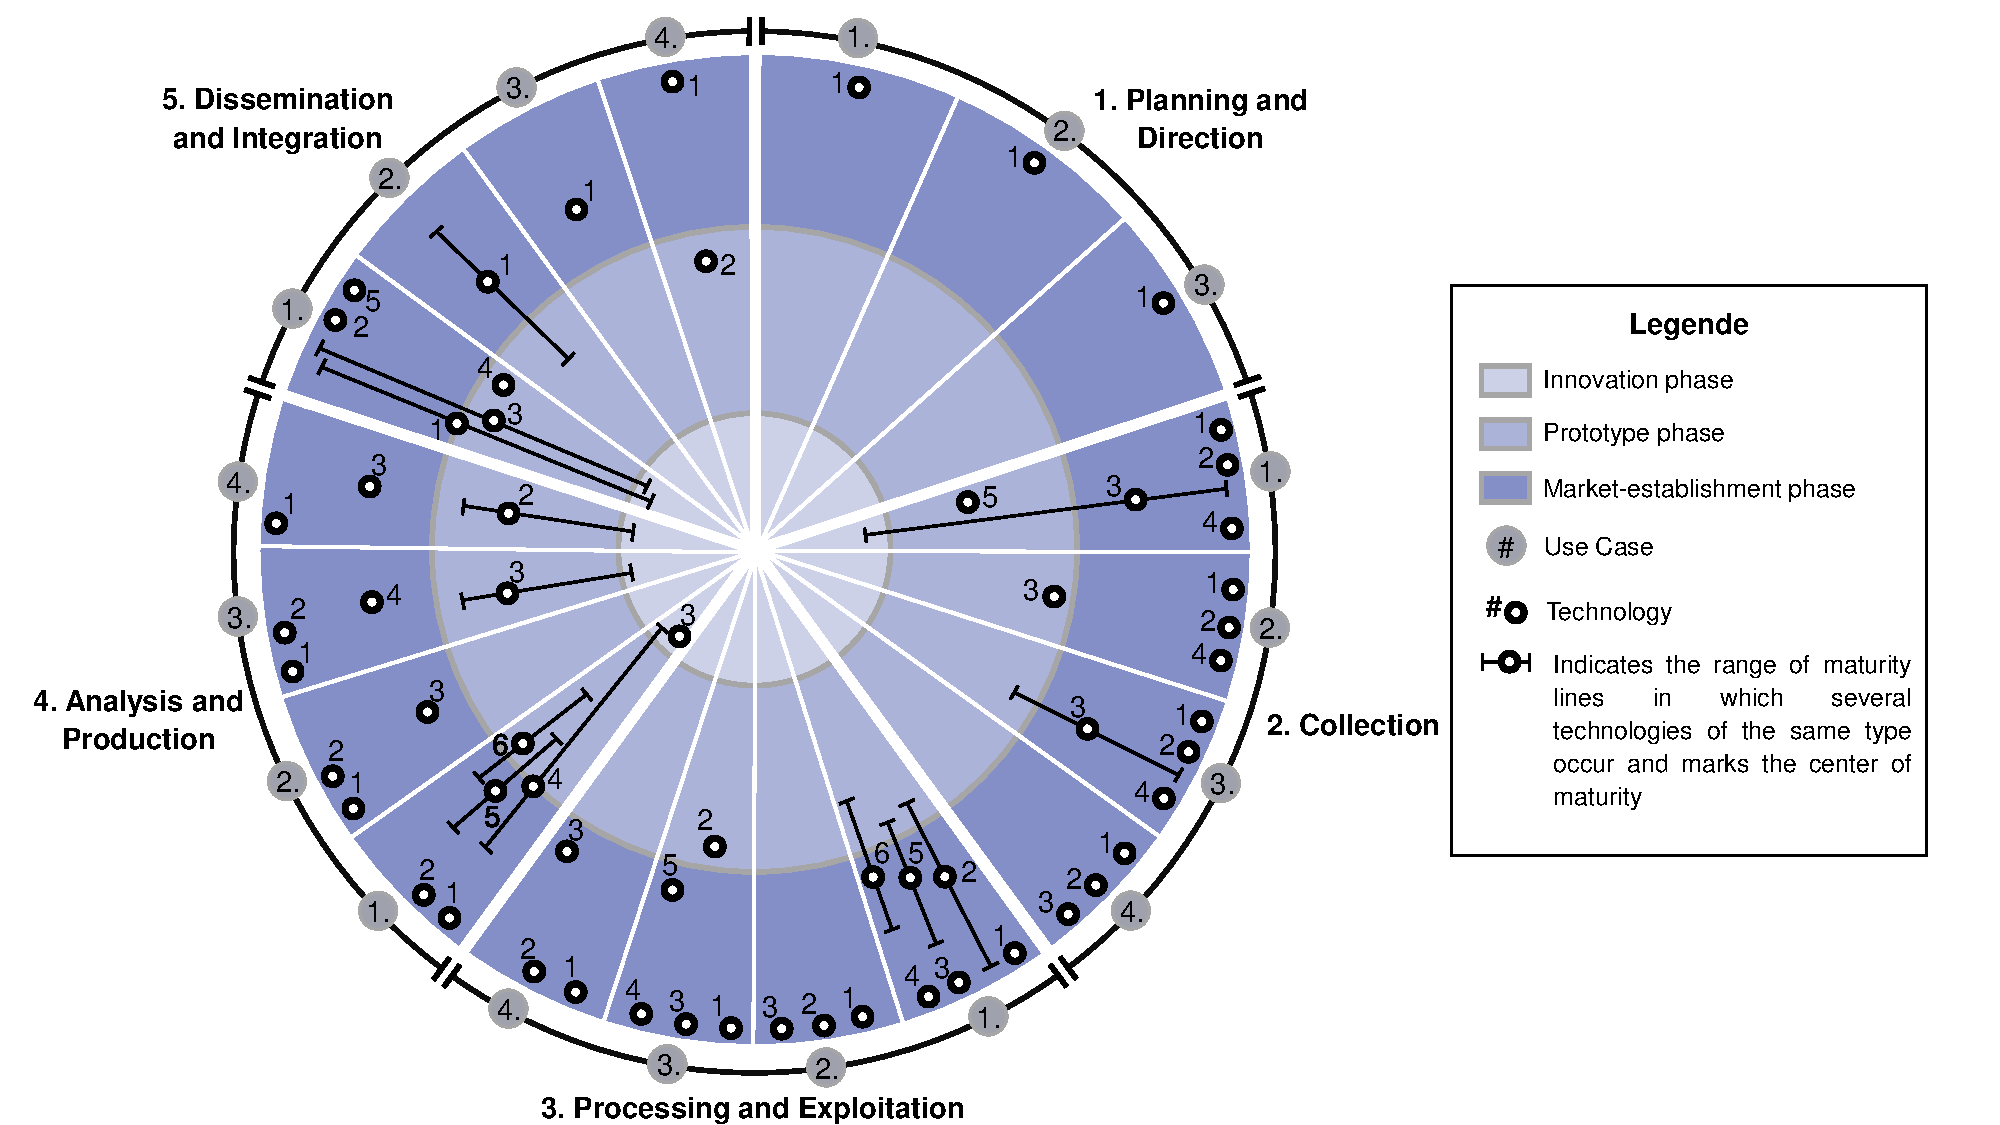
\includegraphics[width=0.7\textwidth]{PDF/images/crop_Trendradar}
    \caption{Resulting Trend Radar based on the Intelligence Cycle}
    \label{fig:trendradar}
\end{figure*}

\begin{figure*}[thb]
    \centering
    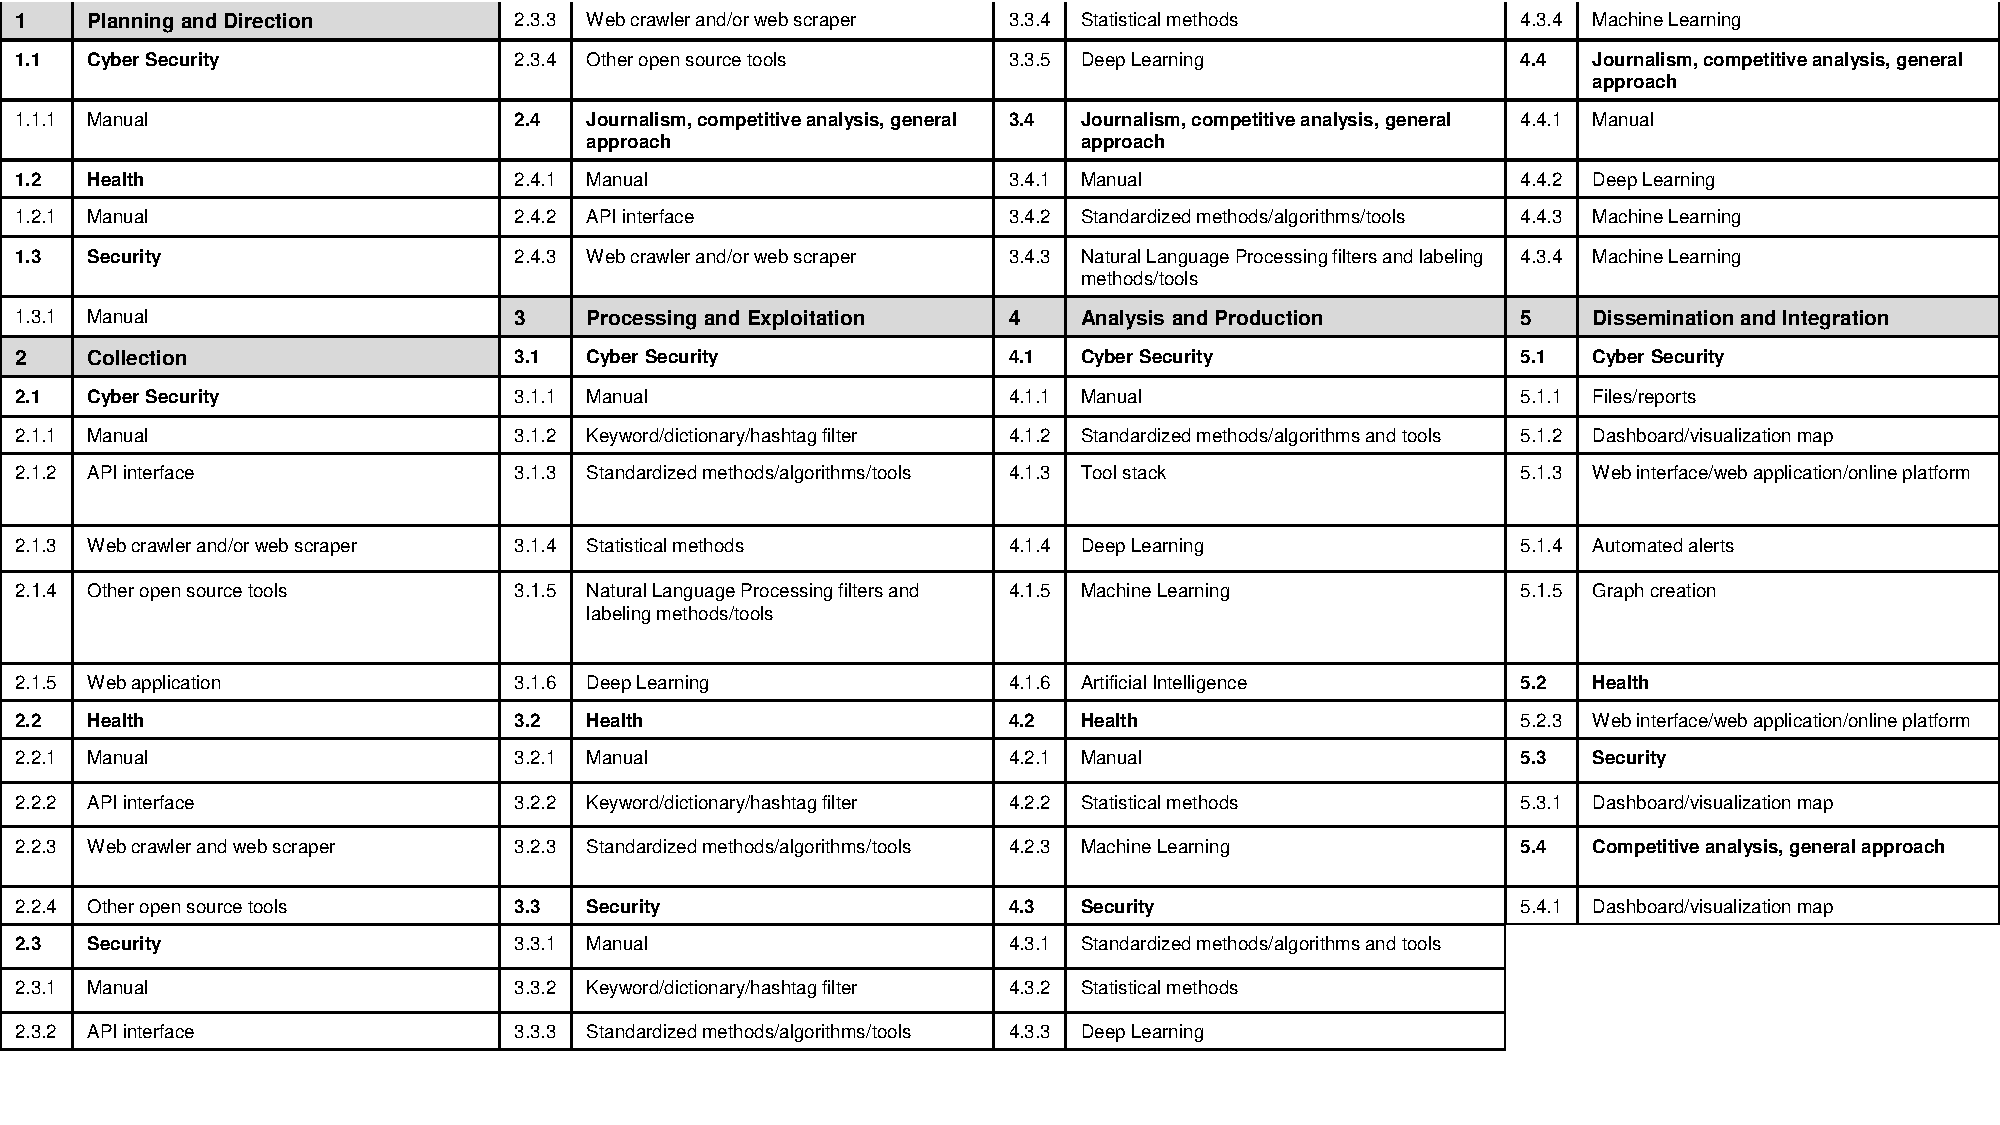
\includegraphics[width=0.99\textwidth]{PDF/images/crop_Trendradar explanation}
    \caption{Content of Trend Radar categorized by Intelligence Cycle phases, use cases, and technologies}
    \label{fig:trendradarexplanation}
\end{figure*}

\subsection{Intelligence Cycle in Theory-Practice Comparison} \label{sec:intcomp}

Studies align with each phase of the IC but no application covers all phases as a third-generation OSINT tool. The literature mainly focuses on the collection phase, followed by analysis/production, and processing/exploitation. The dissemination/integration phase is least covered, followed closely by planning/direction.
These findings align with the experts' practical experiences. They regard the IC as "state of the art" (cf. E3) but note different manifestations of the phases in practice (cf. E4).
The planning/direction phase is often neglected, despite its crucial importance, leading to wasteful production (cf. E3). Conversely, OSINT is frequently associated solely with the collection phase,
resulting in subpar outcomes due to high volumes of low-quality data (cf. E1; E2; E3). The main reason for this is that the IC is operated by at least three groups of people. Firstly, the customers, usually located at the "decision-maker level", with a primarily legal professional background (cf. E2).
The second is the technician who carries out the data collection and processing (cf. E2; E3). Lastly, the analyst evaluates the data and creates the intelligence product (cf. E1). The process thereby is rarely transparent between the parties
(cf. E1; E2) and is rarely anchored at the organizational level (cf. E4). According to the experts, there is thus no third-generation
OSINT tool in use, at least not in German authorities. In addition, the collection focus is driven by concerns about missing vital information, later being revealed as publicly available (cf. E1).

\subsection{Use Cases in Theory-Practice Comparison}

Five main use cases emerged from the research: cyber security, health, security, journalism,
and competition analysis. Cyber security studies primarily focus on Open Source Cyber Threat
Intelligence (OSCTI), which involves collecting, monitoring, and analyzing public
%data to detect potential cyber threats \cite{Ahuja.2022,AlDmour.2023}.
data to detect potential cyber threats (\cite{Ahuja.2022}).
Health applications mainly address COVID-19 outbreak investigations (\cite{Kpozehouen.2020}).
The security use case includes applications such as
analyzing violent behavior in public transport (\cite{Nobili.2021}). The identified journalism study examines the
Twitter activities of the OSINT journalists' association 'Bellingcat' (\cite{Bar.2023}). Competitive analysis
involves, e.g., the performance classification of Chinese logistics companies (\cite{Tao.2023}).
Additionally, two identified studies focus generally on creating knowledge graphs on OSINF (Open Source Information, \cite{Hu.2023, Ma.2022}).

The Experts note that OSINT is used in all authorities and various use cases, even if not explicitly labeled (cf. E2). It is most commonly applied in (cyber) security and OSCTI, especially within German Armed Forces, (Federal) Intelligence Service, domestic intelligence, and police (cf. E1; E2).

\subsection{Technologies and Maturity Levels in Theory-Practice Comparison} \label{sec:matcomp}

Automated technologies are used in all phases and use cases except the initial one. While these technologies exhibit considerable market maturity, manual activities remain prevalent. Particularly cyber security shows the highest level of automation.

The most advanced automated technologies in the collection phase are web crawlers and scrapers. Established tools include 'off-the-shelf' options (cf. \cite{Middleton.2020}) and open-source solutions like 'Tweepy', a Python library for Twitter crawlers (e.g., \cite{Adewopo.2020}). More advanced prototypes combine parallelized, recursive, source-specific web crawlers and scrapers for enhanced data collection (e.g., \cite{Jenkins.2021}). A prototype method called 'focused crawling' adapts the crawling path dynamically using a content-driven ML algorithm, BERT ('Bidirectional Encoder Representation from Transformers', \cite{Kuehn.2023}). Technologies for crawling the dark web, like 'Torsion' (\cite{Sonawane.2022}), belong to the innovation phase. Experts note an increasing use of open-source tools alongside manual work (cf. E1; E3). However, they find traditional web crawling and scraping outdated due to errors and implementation challenges. Screenshot-based 'web shooting' with OCR ('Optical Character Recognition') extraction is seen as more modern and robust (cf. E3).

NLP ('Natural Language Processing') methods such as 'topic classification', 'part-of-speech tagging', and 'entity and relation annotation' demonstrate high automation levels in the processing/exploitation phase. Common technologies include the 'Python NLTK Toolkit' (\cite{Hubbard.2022}) and the 'Stanford CoreNLP Toolkit' (\cite{Middleton.2020}). Additionally, 'Deep Learning' (DL), particularly through 'word embedding' with the 'word2vec' algorithm, is prominent (e.g., \cite{Bai.2020}). Experts note that this phase mainly involves manual work within authorities due to the need for domain knowledge (cf. E1; E2; E3). The degree of automation varies with task abstraction: operational tasks requiring specific information show lower automation than long-term strategic analyses needing extensive data (cf. E3).

The highest automation level is seen in the analysis/production phase, where AI, ML, and DL technologies are prevalent. Under DL, vectorization algorithms, especially BERT versions, are used (e.g., \cite{Ma.2022}). ML models like BERT and 'Supervised Support Vector Machines' (e.g., \cite{Iorga.2020}) are also included, along with 'Random Forests', 'XGBoost', 'lightGBM', 'Naive Bayes', and 'Logistic Regression'. Publications frequently utilize multiple algorithms for performance comparison (e.g., \cite{Tao.2023}) or layered analysis (e.g., \cite{Yang.2022}). AI technologies are less specified, except for \textcite{Dale.2023}, who developed a bidirectional recurrent neural network with BiGur ('Bidirectional Gated Recurrent Unit') layers. Using modular public models, technologies are mainly classified as market-ready. The Experts indicate that this phase largely relies on manual content analysis due to limited technological understanding and acceptance in German authorities (cf. E2; E3; E4). Ethical and legal barriers, like GDPR ('General Data Protection Regulation'), hinder technology adoption (cf. E2; E4). Security concerns favor standalone systems, with smart technologies often used unofficially (cf. E2; E4). However, there is a need for modular, expandable systems to keep pace with advancements (cf. E1; E3; E4). Nonetheless, human experience and specialization are crucial for product quality, while the potential of 'Large Language Models' (LLM) remains uncertain (cf. E4).

In the dissemination/integration phase, tools like 'Power BI' (\cite{Tao.2023}) are used to create dashboards and visualizations. Interfaces, including Python GUIs and browser applications (\cite{Elmas.2022}), along with input masks for entire tool stacks (\cite{Arjun.2020}) are developed. Automated alert technologies for cyber security risk assessments are also common (\cite{Ahuja.2022}), and graph-based visualizations utilize tools/libraries like 'Matplot', 'Networkx', 'Pygraphistry', or the 'Neo4j-Browser' (\cite{Middleton.2020}). Except for alerts, the retrieval of results is largely semi-automated, with technologies in the market establishment phase. No information on user tests or new development involving user feedback was found in any studies. Experts state that automation within authorities during this phase remains very limited. The final product often consists of only a PDF document, email, or verbal report (cf. E1), which suffices in many cases (cf. E3). However, various automated tools beyond OSINT exist that could be applied (cf. E4), and there is a lack of necessary feedback for product improvement in practice (cf. E3).

\section{Discussion and Conclusion} \label{sec:discussion}
%\section{Discussion} \label{sec:discussion}
\subsection{Contributions and Implications}

The investigation into the existence of a robust, automated third-generation OSINT system (e.g., \cite{Ghioni.2023}) concludes negatively for Germany. Identified applications do not fully cover the IC, particularly lacking in the planning/direction and dissemination/integration phases, making human analysis essential. Numerous intelligent tools were identified in other phases, but integration has not met theoretical potential. This finding does not support the thesis of \textcite{Yogish.2021} that automated, AI-driven solutions are indispensable in all OSINT domains. The key research question is why proven applications have not gained widespread use, especially in German intelligence authorities. Future research should also explore enhancing technical support for the initial and final phases of the IC.

%Addressing these questions involves resolving various research gaps (RGs) related to the three key IC groups:
These questions require resolving research gaps (RGs) across the three key IC groups:


%\begin{itemize}
%    \item[\textbf{RG1:}] \textbf{Deficiency in Initial Phase Tools:} There is a technological gap in tools that cover the initial phase of the IC, particularly in frameworks for targeted requirements definition and communication. This gap contributes to an overemphasis on the collection phase \cite{Lowenthal.2020}.
%
%    \item[\textbf{RG2:}] \textbf{Lack of Dissemination Mechanisms:} There is a dearth of effective dissemination and integration mechanisms tailored for authorities, largely due to insufficient user testing and iterative feedback incorporation. The indispensability of consumer feedback is underscored by established frameworks to enhance product quality and reduce data overload \cite{DirectorofNationalIntelligence.2011,JointChiefsofStaffU.S.Army.2013,NorthAtlanticTreatyOrganization.2001,Gibson.2016,Day.2016}.
%
%    \item[\textbf{RG3:}] \textbf{Modular OSINT Systems:} The future of OSINT systems hinges on modular concepts, yet only limited research has been conducted in this area \cite{Arjun.2020,Wright.2020}.
%
%    \item[\textbf{RG4:}] \textbf{Revamping Procurement Procedures:} It's crucial to move away from monolithic stand-alone setups in procurement procedures.
%
%    \item[\textbf{RG5:}] \textbf{Ethical and Legal Compliance:} Ensuring compliance with ethical and legal principles is vital for product adoption, requiring robust legislative updates and considering both national and international regulations, such as GDPR \cite{EuropeanParliament.2016,EuropeanCommission.18.08.2023,Ghioni.2023,Wittmer.2022}.
%
%    \item[\textbf{RG6:}] \textbf{Technical Understanding among Decision Makers:} Addressing challenges necessitates foundational technical understanding at decision-maker levels, fostering openness to technology and cultivating an information-sharing mindset to transcend bureaucratic barriers \cite{NorthAtlanticTreatyOrganization.2001}.
%
%    \item[\textbf{RG7:}] \textbf{Use of LLMs in Intelligence:} While Large Language Models (LLMs) show promise in intelligence analysis, their application in operational settings is underexplored \cite{Radford.2023,Zhao.31.03.2023}.
%
%    \item[\textbf{RG8:}] \textbf{Technological Tools for Technicians:} Technicians often handle significant phases of the Intelligence Cycle independently, yet there is a notable absence of robust collection tools to match the rapidly evolving media landscape.
%
%    \item[\textbf{RG9:}] \textbf{Coordination between Analysts and Technicians:} Coordination gaps between analysts and technicians pose risks of excessive data collection, emphasizing the need for tools that enhance transparency and mitigate collection biases \cite{Lowenthal.2020}.
%\end{itemize}

\setlist{noitemsep}
\begin{itemize}
    \item[\textbf{RG1:}] There is a gap in tools for the initial phase of the IC, in frameworks for requirements definition and communication (Section \ref{sec:intcomp}, cf. E3).
        %This gap contributes to an overemphasis on the collection phase \cite{Lowenthal.2020}.

    \item[\textbf{RG2:}] Effective dissemination and integration mechanisms tailored for authorities are lacking, primarily due to inadequate user testing and feedback incorporation. Established frameworks emphasize the importance of consumer feedback for product quality and data overload mitigation (\cite{JointChiefsofStaffU.S.Army.2013, NorthAtlanticTreatyOrganization.2001}).

    \item[\textbf{RG3:}] The future of OSINT systems relies on modular concepts, yet research in this area is limited (\cite{Arjun.2020,Wright.2020}).

    \item[\textbf{RG4:}] It is crucial to move away from monolithic stand-alone setups in procurement procedures (Section \ref{sec:matcomp}, cf. E1; E3; E4).

    \item[\textbf{RG5:}] Ensuring compliance with ethical and legal principles is vital for product adoption, necessitating robust legislative updates and adherence to regulations like GDPR (\cite{EuropeanParliament.2016, Wittmer.2022}).

    \item[\textbf{RG6:}] Addressing challenges requires a foundational technical understanding among decision-makers to foster openness to technology and enhance information sharing (\cite{NorthAtlanticTreatyOrganization.2001}).

    \item[\textbf{RG7:}] While LLMs show promise in intelligence analysis, their operational application remains underexplored (\cite{Radford.2023}).

    \item[\textbf{RG8:}] Technicians often work independently in the IC, yet there is a lack of robust collection tools to match the rapidly evolving media landscape (Section \ref{sec:matcomp}, cf. E4).

    \item[\textbf{RG9:}] Coordination gaps between analysts and technicians risk excessive data collection, showing a need for tools to improve transparency and mitigate biases (\cite{Lowenthal.2020}).
\end{itemize}
%These gaps highlight the critical areas for future development and research to enhance the efficiency and effectiveness of intelligence operations.

\subsection{Limitations and Future Research}

The first limitation is the lack of clarity regarding the legal and ethical basis (\cite{Ghioni.2023,Wittmer.2022}), preventing verification of whether only public sources (\cite{NorthAtlanticTreatyOrganization.2002}) were used in the analyzed studies. Additionally, it was not confirmed whether the technologies met the legal and ethical requirements for the use of the information obtained (\cite{PastorGalindo.2020,Wittmer.2022}).

The second limitation arises from classification categories not fully aligning with the MECE (Mutually Exclusive and Collectively Exhaustive) principle (\cite{Lee.2018}), particularly regarding the hierarchical dependency of AI, ML, and DL technologies. While the authors' wording was followed for objective reproduction, the accuracy of the information was not reviewed in detail. Furthermore, no fixed limits could be defined for the volume category, as these were not uniformly recorded in the studies.

The third limitation involves the small sample size of expert interviews, which were confined to Germany. Due to the difficulty in accessing this target group, interviews were not conducted with active users and decision-makers within authorities. Independent verification of coding by a second researcher is also recommended for improved intercoder reliability (\cite{Glaser.2009}). Lastly, the research followed a linear execution rather than the suggested iterative approach (\cite{Peffers.2007}).

Despite these limitations, this study provides a comprehensive OSINT knowledge base through a practice-evaluated TR. It introduces a structured mechanism for capturing rapid developments and sheds light on the public security sector. Moreover, it serves as a guide for practitioners. Initial evaluations reveal two unanswered research questions and nine research gaps, highlighting critical areas for further exploration. Future research could apply this framework in other countries, where intelligence agencies may have more digitized processes, such as in allied nations (cf. E2). Extending the framework to other intelligence disciplines or domains, like the medical sector, could also offer new opportunities (cf. E4). The TR aims to elevate OSINT within academic research as an essential tool in today’s complex world.


%This study offers a comprehensive knowledge base on OSINT through a field-evaluated trend radar. The radar identifies key use cases, technologies and thier characteristics, introducing a mechanism that captures the subject's rapid evolution and ensures temporal persistence. It also provides new insights into the public security sector, previously underexplored due to access challenges. Initial evaluations reveal two unanswered research questions and nine research gaps, highlighting critical areas for further development. Future research could apply this framework to other countries, where intelligence agencies may have more advanced, (digitized) processes, such as in allied nations (cf. E2). Extending the framework to other intelligence disciplines or domains like the medical sector, where similar digitized processes exist (cf. E4), could also offer new study opportunities. The trend radar serves as a practical guide for practitioners, and it is hoped that this study will elevate OSINT in academic research, enhancing this essential tool in today’s dangerous world.

%Nevertheless, the study furnishes future researchers with a comprehensive knowledge base on OSINT
%through a practice-evaluated artifact, a trend radar.
%The radar serves as a comprehensive knowledge base, allowing for contemporary evaluation and analysis of OSINT technologies.
%Initial evaluations reveal two crucial unanswered research questions and identify nine detailed research gaps, highlighting
%critical areas for future development and research to enhance the efficiency and effectiveness of intelligence operations.
%as well as identifying research gaps for future studies, penetrating the complex research field. 
%Moreover, the developed trend radar serves as a guideline for practitioners. The radar
%is adaptable to the evolving subject area and transferable to other intelligence disciplines. Hopefully, the findings of this study can give OSINT some traction in the academic research context to augment and improve a very important tool in today’s dangerous world.


%Before addressing these questions, future researchers are advised to validate them further. 
%Utilizing the presented tools to reevaluate literature
%categorization and update identified technologies is recommended. In addition, semantic
%control and indexing methods (e.g. LLM) should be included. Due to the high dynamic of the research field,
%it is also recommended to integrate news articles and scientific journals with shorter publication cycles.
%Reassessing categories based on MECE criteria and conducting further interviews, including internationally
%and with active authority members, is advisable. Employing methods like the Delphi technique to evaluate
%trends and establish consensus is suggested \cite{Hader.2000}. Subsequent iterations of the design process and adjustments
%to the trend radar, if necessary, should follow based on these results \cite{Peffers.2007,Sonnenberg.2012}.

%\subsection{Conclusion}
%\subsection{Summary}

%In this paper, a practice-validated trend radar was developed that depicts current trends
%in the field of OSINT through applied technologies. It serves as a comprehensive knowledge base,
%allowing for contemporary evaluation and analysis of OSINT technologies as well as identifying research
%gaps for future studies, penetrating the complex research field. Moreover, it serves as a guideline for practitioners. The radar
%is adaptable to the evolving subject area and transferable to other intelligence disciplines.
%Based on the developed trend radar, current research gaps are identified and new research questions are raised.

%Results reveal the absence of an automated third-generation OSINT system in Germany, highlighting the
%need for technological support in the planning and direction as well as the dissemination and integration phases.
%The research questions identified for future studies are therefore, why proven, available applications,
%have not yet found widespread use, especially in the security authorities.
%In addition, the question of how the first and last Intelligent Cycle phases, alongside the others,
%can be better supported technically is to be investigated. The research gaps identified extend
%not only to technology but in particular to the legal, administrative, political and
%social sciences, necessitating interdisciplinary collaboration. Above all, a need to catch up is seen
%in the non-technical research fields, responsible for creating the decisive prerequisites for technology
%implementation.


% Fonts specification --- not shown as it doesn't exist in the Word document either. 

%\section{Fonts}

%A summary of fonts is provided in Table \ref{tab: fonts}. 

%\begin{table}[thb]
%\centering
%\caption{\label{font-table} Font guide. \vskip 3pt }
%\label{tab: fonts}
%\begin{tabular}{l|rl}
%\hline \bf Type of Text & \bf Font Size & \bf Style \\ \hline
%paper title & 14 pt &  \bf bold \\
%authors & 10 pt &  \underline{email} underlined \\
%abstract title & 12 pt &  \bf bold\\
%abstract text & 10 pt &  \it italic\\
%section titles & 12 pt & \bf bold \\
%subsection titles & 11 pt & \bf bold \\
%document text & 10 pt  & \\
%captions & 9 pt & \sansserifformat{\captionsize sans-serif, \bf bold} \\
%bibliography & 9 pt & \\
%footnotes & 8 pt & \\
%\hline
%\end{tabular}
%\end{table}


% \section{References}


%Bibliography 

%\bibliographystyle{ieeetr}
%\bibliography{references}


%Bibliography 


\printbibliography

\end{document}
